\documentclass[../EDF Master Thesis.tex]{subfiles}

\begin{document}

Als Plattform für dieses Projekt dient ein STM32F769I-Disc0 Board der Firma ST, welcher unter anderem folgende Hauptmerkmale besitzt:

\begin{itemize}
    \item Prozessor: ARM®Cortex®-M7
    \item ROM: 2 Mbytes
    \item RAM: 532 Kbytes
    \item Schnittstellen:
    \begin{itemize}
        \item Ethernet-Schnittstelle
        \item Zwei Push-Buttons
        \item 7 One-Board \ac{led}s
    \end{itemize}
\end{itemize}


Dieses ist mit einen ARM®Cortex®-M7 Prozessor ausgestattet und hat für die verwendete Arbeit und erarbeiteten Demo-Applikationen ausreichende Rechenleistung.
Für die Kommunikation zwischen Host-Computer und Mikrocontroller wurde die integrierte Ethernet Schnittstelle verwendet.
Für die 'Blinky-Demo' wurden außerdem die drei, auf dem Board integrierten, \ac{led}s verwendet.

\begin{figure}[ht!]
    \begin{center}
        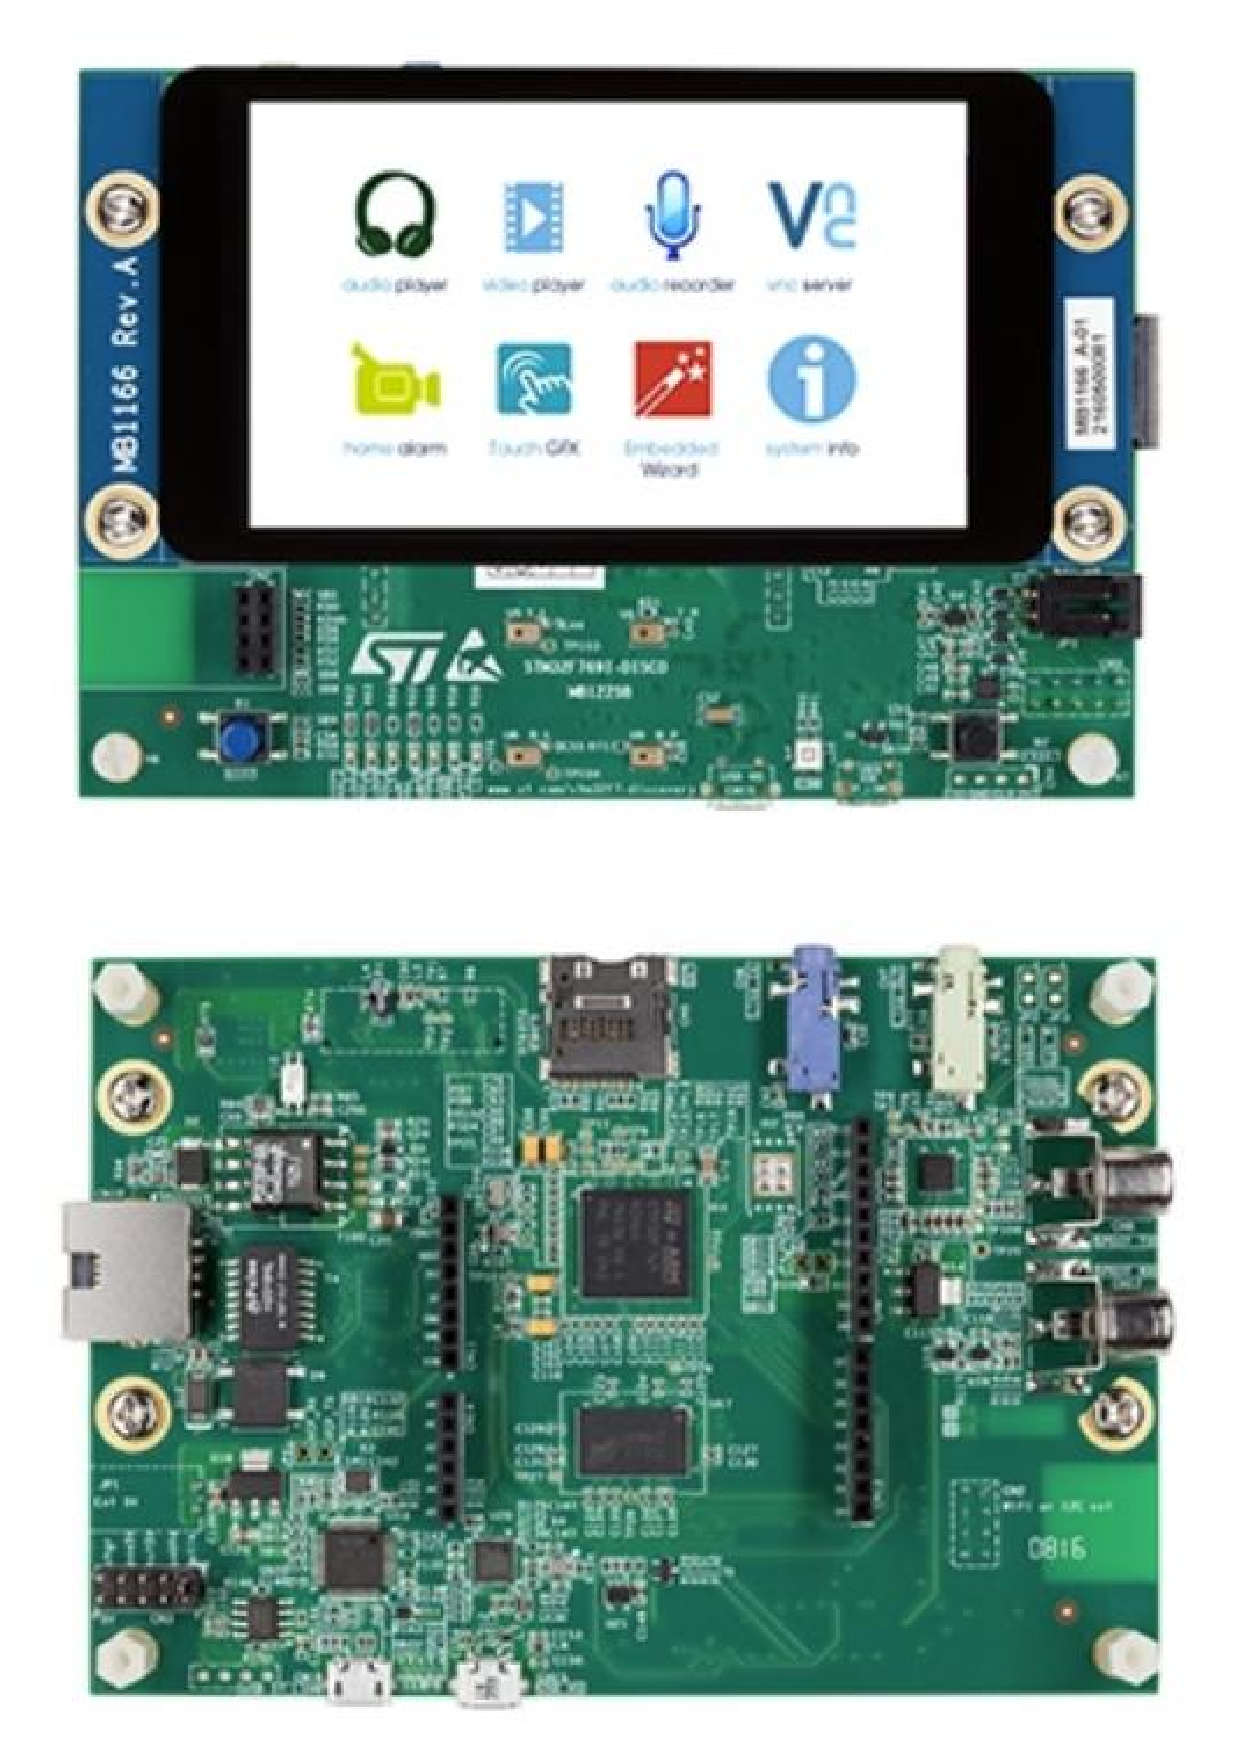
\includegraphics[width=0.6\textwidth]{attachments/stm32f769i-disc0.pdf}
    \end{center}
    \caption[STM32F769I-Disc0 Board]{STM32F769I-Disc0 Board (Quelle: \cite{stm:001})}
    \label{fig:STM32F769I-Disc0_board}
\end{figure}

\end{document}
